\documentclass[oneside,12pt]{book}
\usepackage[utf8]{inputenc}
\usepackage{standalone}
\usepackage[margin=2.5cm]{geometry}
\usepackage{graphicx}
\usepackage{hyperref}
\usepackage{lmodern}
\usepackage{float}
\usepackage{csquotes}
\usepackage[figurename=Ilustración]{caption}
\usepackage[numbers]{natbib}
\usepackage{ragged2e}
\usepackage{array}
\usepackage{multirow}
\usepackage{parskip}
\usepackage{listings}
\usepackage{epigraph}
\usepackage{lipsum} % Texto de relleno en plantilla

\usepackage{comment} %Uso de comentarios multilínea

%\usepackage{fancyhdr}
\usepackage{geometry}
\usepackage{color}\usepackage{graphicx,xcolor}

\usepackage{titlesec}
\setcounter{secnumdepth}{3}
\titleformat{\chapter}[display]
{\normalfont\huge\bfseries}{\chaptertitlename\ \thechapter}{20pt}{\Huge}

\urlstyle{same}
\title{Galería de NFT's en la Web3}
\author{Cristóbal José Jiménez Gómez}
\date{Curso 2022 - 2023}
\renewcommand{\contentsname}{Contenido}
\renewcommand{\figurename}{Ilustración}
\usepackage{pifont}
\renewcommand\labelitemi{\ding{52}}

%Corrección de idioma
\usepackage[spanish,es-tabla]{babel}

%Agregados por mi%
%para la bibliografía%
\usepackage{natbib}
\bibliographystyle{unsrtnat}

%Para las tablas
\usepackage{tabularx}

%Para las imágenes
\usepackage{graphicx}

%Colores 
\usepackage{xcolor}

\begin{document}
\begin{titlepage}
    \begin{center}
    \vspace*{0.5in}
        \begin{figure}[htb]
            \begin{center}
            
\includegraphics[width=15cm]{Ilustraciones/LogoEII.jpg}
            \end{center}
        \end{figure}

        \vspace*{0.15in}
        \vspace*{0.2in}

        \noindent\hfil\rule{11cm}{0.2mm}\hfil\\
        \vspace*{0.1in}
        \begin{Huge}
            \textbf{Galería de NFT's en Web3} \\
        \end{Huge}

        \vspace*{0.3in}

        \begin{large}
            TITULACIÓN: Grado en Ingeniería Informática \\
            \vspace*{0.1in}
            AUTOR: Cristóbal José Jiménez Gómez \\
        \end{large}
        \vspace*{0.3in}
        
        \noindent\hfil\rule{11cm}{0.2mm}\hfil\\

        \vspace*{0.1in}

        \begin{large}
            TUTORIZADO POR: \\
            María Dolores Afonso Suárez \\
        \end{large}
        
    \vspace*{0.3in}

    Fecha: 05/2023
    \end{center}
\end{titlepage}


%\newgeometry{margin=1.5cm}

\thispagestyle{empty}

%\lhead{ 
\begin{tabular}{p{15cm}p{5cm}}
  
\includegraphics{Ilustraciones/LogoEII.jpg}   &  TFT04\\
\end{tabular}
%}

\vspace{1em}
\fboxrule=2pt
\begin{center}
\fcolorbox{gray}{gray!10}{\parbox{.8 \textwidth}{ {\large SOLICITUD DE DEFENSA DE TRABAJO DE FIN DE TÍTULO}}}
\end{center}

\vspace{1em}
\justify
D./Dª Nombre\_Estudiante, autor del trabajo Título\_Trabajo, correspondiente a la titulación Titulación\_Estudiante, en colaboración con la empresa/proyecto Nombre\_Empresa (en su caso)

\vspace{1em}
SOLICITA

\vspace{1em}
que se inicie el procedimiento de defensa del mismo, para lo que se adjunta la documentación requerida, haciendo constar que 

[ ] se autoriza / [ ] no se autoriza la grabación en audio de la exposición y turno de preguntas.

\vspace{1em}
Asimismo, con respecto al registro de la propiedad intelectual/industrial del TFT, declara que:

[ ] Se ha iniciado o hay intención de iniciarlo (defensa no pública).

[ ] No está previsto.

\vspace{1em}
Y para que así conste firma la presente. (fecha en firma electrónica)

\begin{center}
%En Las Palmas de Gran Canaria, a día de mes de año

\vspace{1em}
El/La estudiante

\vspace{3em}
Fdo.------------------------
\end{center}

\begin{center}
\fcolorbox{gray}{white!10}{\parbox{.9\textwidth}{
{\tiny A rellenar y firmar \textbf{obligatoriamente} por el/la/los/las tutores}

En relación con la presente solicitud, se informa:{\tiny (firmar donde corresponda)}

\vspace{1em}
\begin{center}
\begin{tabular}{|p{\dimexpr.45\linewidth}|p{\dimexpr.45\linewidth}|}
%\begin{tabular}{|l|r|}
    \hline
   & \\
  Positivamente {\tiny (en  caso  de  detección  de  copia, esta firma quedará invalidada)}  & Negativamente {\tiny (justificación en TFT05)} \\
   & \\
   & \\
   & \\
   & \\
   & \\
   & \\
  Fdo.------------------------ & Fdo.------------------------  \\
     & \\

    \hline
\end{tabular} 

\end{center}

\vspace{1em}

}
}

\vspace{1em}

%\cfoot{
DIRECTORA DE LA ESCUELA DE INGENIERÍA INFORMÁTICA
%}

\end{center}

\restoregeometry

\clearpage

\newpage
\pagenumbering{arabic}
{\Large{\textbf{Agradecimientos}}}

\begin{flushright}
    {\setlength{\parskip}{8mm}
        \large{
            \textit{A los gnomos de jardín.}
        }
    }
    
\end{flushright}

\clearpage
{\setlength{\parskip}{8mm}
{\huge{\textbf{Resumen}}}

    {\large{ 
        Desarrollo de una Aplicación Web en el marco de la Web3(blockchain), que gestiona una galería de 
        Non Fungible Tokens (NFT’s). Ofrece la gestión de contenidos a distintos tipos de usuarios cuyos niveles de
        interacción varían desde los usuarios sin registrar, a administradores. En esa escala de accesos los
        casos de uso establecerán el nivel de interacción de cada perfil. Las funcionalidades implementadas
        permitirán la gestión a distintos niveles de estos NFT’s, desde la visualización hasta la gestión de cada
        cartera. Este último concepto es el definido para almacenarlos y, en caso de ser necesario comerciar
        (compraventa o intercambio) con ellos.
    }}

    \textbf{Palabras claves:} Web3, Web3.0, Angular, Firebase, Vercel, Express
    

%\newpage

{\huge{\textbf{Abstract}}}

    {\large{
        Development of a Web Application within the framework of Web3 (blockchain), which manages a gallery of
        Non Fungible Tokens (NFT's). It offers content management to different types of users whose levels of
        Interaction range from unregistered users to administrators. At this access scale, the
        use cases will establish the level of interaction of each profile. The functionalities implemented
        will allow the management at different levels of these NFTs, from the visualization to the management of each
        briefcase. This last concept is the one defined to store them and, in case it is necessary to trade
        (purchase or exchange) with them.
    }}

    \textbf{Key Words:} Web3, Web3.0, Angular, Firebase, Vercel, Express
} 
\tableofcontents
\newpage
\listoffigures
\newpage
\listoftables

\clearpage
\pagenumbering{arabic}

%----Introducción----%
%--Motivación/Objetivos/Estructura de memoria--%
\chapter{Introducción}
\section{Motivación}
La razón principal que se encontró para la elaboración de este trabajo ha sido 
el auge de la Blockchain durante estos últimos años. "Blockchain es un libro 
mayor compartido e inalterable que facilita el proceso de registro de 
transacciones y de seguimiento de activos en una red de negocios. Un activo 
puede ser tangible o intangible. Prácticamente cualquier cosa de valor, puede 
rastrearse y comercializarse en una red de blockchain, reduciendo así el 
riesgo y los costes para todos los involucrados"\cite{ibmWeb3}. 

Esta tecnología ofrece la posibilidad de cosntruir aplicaciones web que garanticen
la privacidad y seguridad de los datos de un usuario. La Web 3 ofrece transparencia
y trazabilidad a la hora de la interacción entre usuarios. Además, permite la 
creación o conversión de negocios ya afianzados a este entorno.

Además, se afianza una necesidad que encontraba yo, personalmente, a la hora de
interactuar entre distintas carteras, que es la necesidad de tener todas en una 
misma ubicación.

Se debe constar que ya existen páginas afianzadas para el fin de mostrar y 
compra-venta de NFT's. Este trabajo busca el aprendizaje tanto del desarrollo 
de una aplicación web completa, como de aprender a realizar las llamadas y 
conexiones para recoger y mostrar datos de NFT's\cite{bbcNFTs} y 
criptocarteras\cite{moralisWallets}.

\newpage
\section{Objetivos}
El objetivo principal del proyecto se centra en el desarrollo de un sitio web 
que utiliza el nuevo concepto de descentralización dentro del marco Web3. 
El resultado ofrece como funcionalidad principal la búsqueda de NFT’s y el 
almacenamiento de distintas carteras de criptomonedas. Para ello se plantea 
un conjunto de objetivos generales:
\begin{enumerate}
    \item Estudiar las características y evolución de la Web 3.0 y su relación con la Web3.
    \item Realizar un estudio de las tecnologías y herramientas a emplear.
    \item Establecer criterios para su selección (tanto las tecnologías como de las herramientas)
    \item Seguir una metodología de desarrollo, las pruebas y documentación del proyecto.
\end{enumerate}




\section{Estructura de la memoria}
La memoria está dividida en 10 capítulos diferentes. En ellos se recoge toda
la información, desde el inicio del proyecto hasta las conclusiones. Así, 
la información recogida en cada capítulo se describe tal que:

\-\hspace{1cm} El primer capítulo consta de la introducción al proyecto. En este se 
contextualiza el trabajo, se explica la motivación detrás de la elaboración 
del proyecto, se dan a conocer los objetivos a cumplir y se explica la 
estructura del documento.

\-\hspace{1cm} El segundo capítulo lista y justifica las competencias de la titulación
abarcadas durante el desarrollo del trbajo mediante las teras y actividades realizadas.

\-\hspace{1cm} El tercer capítulo desarrolla el marco teórico, donde se explican y 
analizan algunos términos relevantes a este trabajo. Es el punto de partida, 
donde se realiza una investifación que contextualiza y justifica las cacciones
que se toman en el trabajo.

\-\hspace{1cm} El cuarto capítulo abarca el estado del arte, que explica la 
actualidad del desarrollo Web junto con el desarrollo dentro de la Web3.0 y 
la popularidad entre los distintos frameworks\footnote{Un framework es una 
herramienta de programación que te permite desarrollar software proporcionando 
una estructura con componentes integrados que sirven de base para construir 
proyectos nuevos\cite{bootcampFramework}}

\-\hspace{1cm} El quinto capítulo contiene los recursos y las tecnologías 
utilizadas para el desarrollo del trabajo. En este se definen y justifican.

\-\hspace{1cm} El sexto capítulo se explica la metodología llevada a cabo 
para la realización del trabajo, se dan a conocer als diferentes fases y 
tareas que han existido durante su desarrollo.

\-\hspace{1cm} El séptimo capítulo se incluye un análisis de los requisistos y 
el diseño de la página que se ha elaborado para el desarrollo.

\-\hspace{1cm} El octavo capítulo se explica todo lo relacionado con el 
desarrollo de la página web.

\-\hspace{1cm} El noveno capítulo se encuentra la evaluación de la calidad de la página, 
obtenidos a través de diversos programas o extensiones.

\-\hspace{1cm} El décimo capítulo se incluye las conclusiones que se pueden obtener 
de este proyecto, tanto personales como objetivas, dando además una propuesta de mejora 
para un futuro desarrollo.

\-\hspace{1cm} Finalmente se incluyen los anexos, los cuales también contienen las 
referencias bibliográficas


\newpage
%----Competencias----%
\chapter{Competencias específicas}
Las competencias aplicadas a este proyecto se pueden encontrar en la Tabla 
\ref{tab:competencias} y a continuación se listan: CI8, CI13, CI16, CI17, T12.\\
\-\hspace{1cm} La competencia CI8 se justifica debido a la necesidad de analizar,
diseñar y construir los distintos componentes de la página web, así como las 
estructuras de los distintos documentos de la base de datos.\\
\-\hspace{1cm} La competencia CI13 se justifica por el uso de hacer llamadas a API's
y la creación de un backend. Así como a la hora de desplegar la aplicación a internet. \\
\-\hspace{1cm} La competencia CI16 se justifica debido a la metodología Scrum aplicada
durante el transcurso del proyecto. \\
\-\hspace{1cm} La competencia CI17 se justifica gracias al uso de los programas de 
caldiad utilizados para garantizar la accesibilidad y usabilidad de la página web.\\
\-\hspace{1cm} La competencia T12 se justifica debido a que en eso ha consistido este proyecto: \\
\-\hspace{1.5cm} \textbf{Diseño} de los distintos componentes y páginas de la aplicación.\\
\-\hspace{1.5cm} \textbf{Despliegue} de la aplicación en sus diferentes ramas para poder ser \textbf{evaluadas} 
    por distintos usuarios.\\
\-\hspace{1.5cm} \textbf{Selección} de las herramientas como pueden ser el \textit{framework} sobre el que se ha 
trabajado (Angular), o la página sobre la que se ha hecho el \textit{despliegue}, siempre teniendo en \textit{cuenta el coste 
y la calidad} del mismo.\\

\begin{table}[H]
    \caption{\textbf{Competencias} cubiertas durante el desarrollo del proyecto.}
    \hfill \break
    \label{tab:competencias}
    \begin{tabularx}{\linewidth}{| @{} >{\bfseries}l | >{\RaggedRight}X @{} | }
        \hline
        \centering \textbf{Código} & \textbf{Descripción} \\
        \hline
        CI8  & Capacidad para analizar, diseñar, construir y mantener 
        aplicaciones de forma robusta, segura y eficiente, eligiendo el 
        paradigma y los lenguajes de programación más adecuados. \\ 
        \hline
        CI13 & Conocimiento y aplicación de las herramientas necesarias para el 
        almacenamiento, procesamiento y acceso a los sistemas de 
        información, incluidos los basados en web. \\ 
        \hline
        CI16 & Conocimiento y aplicación de los principios, metodologías y ciclos 
        de vida de la ingeniería del Software \\
        \hline
        CI17 & Capacidad para diseñar y evaluar interfaces persona computador que 
        garanticen la accesibilidad y usabilidad a los sistemas, servicios y 
        aplicaciones informáticas. \\ 
        \hline
        T12  & Capacidad para seleccionar, diseñar, desplegar, integrar, evaluar, 
        construir, gestionar, explotar y mantener las tecnologías 
        de hardware, software y redes, dentro de los parámetros de coste y 
        calidad adecuados.\\ 
        \hline
    \end{tabularx}
    \hfill \break
    \hfill \break
    \centering\textbf{Fuente:} Universidad de Las Palmas de Gran Canaria (2023)
\end{table}
\newpage
%----Estado actual y Objetivos iniciales----%
%--Objetivos iniciales/Estado actual--%
\chapter{Objetivos iniciales y estado actual}
El principal objetivo de este Trabajo de Fin de Grado se centra en el
desarrollo de un sitio que que hace uso del nuevo concepto de descentralización
dentro del marco de la web 3.0 (Ver la evolución de la web en la sección
\ref{txt:web3}).

El resultado ofrece como funcionalidad principal la búsqueda de NFT's (Ver la
descripción en la sección \ref{txt:nft}) y el almacenamiento de distintas
carteras de criptomonedas (Ver la descripción en la sección \ref{txt:wallet}).

Para ello se plantea un conjunto de objetivos generales:
\begin{enumerate}
    \item Estudiar las características y evolución de la Web 3.0 y su relación con la
          Web3.
          \begin{itemize}
              \item Como se puede ver en el Capítulo 4, se han estudiado tanto las características,
                    como la evolución de las Web3, sus diversos usos en la actualidad.
          \end{itemize}
    \item Realizar un estudio de las tecnologías y herramientas a emplear.
          \begin{itemize}
              \item Firebase es una de las principales herramientas de Google para el manejo de
                    usuarios
              \item Hay una gran cantidad de API's que nos ayudan a acceder a la Web3, entre ellas:
                    \begin{itemize}
                        \item Coinbase: \url{https://docs.cloud.coinbase.com}
                        \item ThirdWeb: \url{https://thirdweb.com}
                        \item Moralis: \url{https://moralis.io}
                        \item Alchemy: \url{https://www.alchemy.com}
                    \end{itemize}
              \item Para el backend se revisó el uso de Django y de Express.js:
                    \begin{itemize}
                        \item Usé Django en las Prácticas Externas y pude ver que es de fácil uso y
                              comprensión debido al uso de Python, pero eran necesarios demasiados pasos para
                              el despliegue de la aplicación
                        \item Con Express.js fue simple, ya que ejecutar un servidor que escuche un puerto en
                              concreto, es la base del funcionamiento de este Framework
                    \end{itemize}
              \item Para desplegar la página se ha revisado el funcionamiento de Amazon Web
                    Service, GitHub Pages y Vercel:
                    \begin{itemize}
                        \item Amazon Web Services es multiusos, lo vi como "matar una mosca a cañozazos",
                              algo demasiado grande para lo que iba a ser el proyecto
                        \item A la hora de desplegar un proyecto angular en GitHub Pages me resultó
                              complicado, ya que se tenía que crear la build del proyecto, y luego asignar el
                              fichero que se mostraba. Si en algún momento me olvidaba de hacer una build, no
                              se actualizaba aquí, por lo que fue descartada
                        \item Vercel aportaba algo simple, ya que si era un proyecto Angular lo desplegaba
                              directamente, y a la hora de desplegar el backend, hecho en Express.js resultó
                              ser sencillo, con un fichero de configuración escrito gracias a la
                              documentación de Vercel
                    \end{itemize}
          \end{itemize}
    \item Establecer criterios para su selección (tanto las tecnologías como de las
          herramientas) Este apartado se comprobará mejor en el Capítulo \ref{recursos}
          \begin{itemize}
              \item Debido al "poco tiempo de desarollo" decidí escoger las herramientas según la
                    complejidad de las mismas:
                    \begin{itemize}
                        \item Para tener la información de los usuarios, las distintas colecciones a mostrar,
                              etc. Se usó Firebase por ser de Google y de las más completas
                        \item Para la obtención de NFT's se hizo uso de la API Alchemy, que con la
                              documentación que se encontraba en la web se hizo fácil de usar
                        \item Para la obtención del balance de las carteras a partir de su dirección pública
                              se hizo uso de la API de Moralis, ya que pude encontrar diversas formas de
                              hacerlo, pero esta fue la más efectiva
                        \item Para esta última parte se hizo un backend con Express.js, que nos permite hacer
                              uso de la funcionalidad de JavaScript para hacerlo
                        \item Para el despliegue de la aplicación se hizo uso de Vercel, por su simplicidad a
                              la hora de desplegar los proyectos y documentación
                    \end{itemize}
          \end{itemize}
    \item Seguir una metodología de desarrollo, las pruebas y documentación del proyecto.
\end{enumerate}
\newpage
%----Fin de introducción----%
%----Desarrollo como concepto----%
\chapter{Marco teórico}
En esta parte del informe se darñan los conceptos generales para la comprensión del mismo.
Se hará un paso por la historia de la Web desde sus inicios hasta como la conocemos ahora 
y se darán los conocimientos básicos para comprender el funcionamiento de las criptomonedas,
los Token's no fungibles y las criptocarteras.
\section{Historia de la Web hasta la Web 3.0}
\label{txt:web3}
La \textbf{World Wide Web} fue creada en 1989 por el científico británico 
\textit{Tim Berners-Lee} mientras trabajaba en el \textit{Centro Europeo de Investigación 
Nuclear(CERN)}. La idea era crear una red de información que pudiera ser compartida 
entre científicos y académicos de todo el mundo. Para evitar un apagado accidental se escribió 
una nota en tinta roja (Figura \ref*{fig:cern-server}) que ponía: "\textcolor{red}{This machine is a server. DO NOT 
POWER IT DOWN!!}"\cite{cernWeb1} (Esta máquina es un servidor. ¡¡NO LO APAGUEN!!) \\
\begin{figure}[htb!]
    \caption{Pegatina del servidor del CERN con la WWW}
    \label{fig:cern-server}
    \centering
    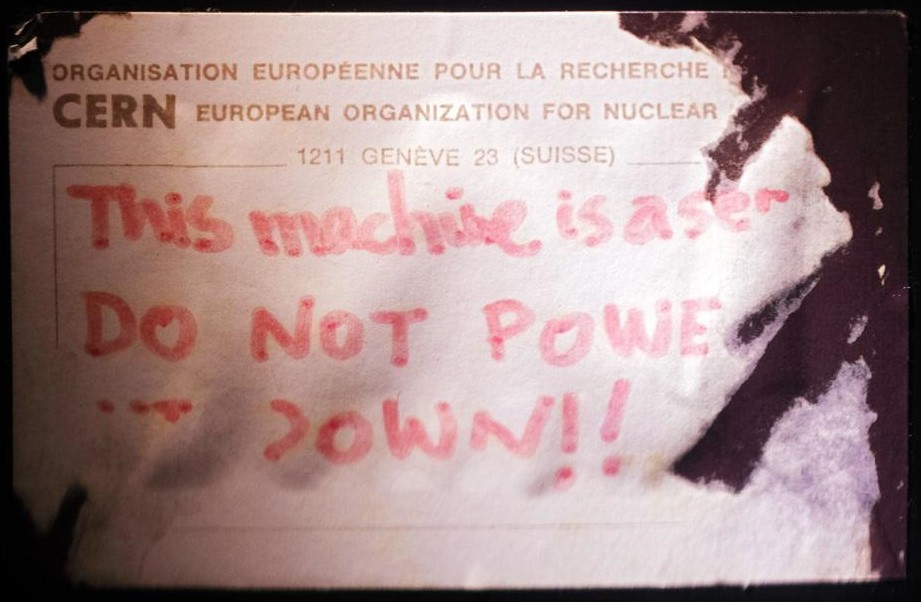
\includegraphics[scale=0.25]{./Ilustraciones/cern-server.jpg}\\
    \textbf{Fuente:} Reddint oficial del CERN [\url{https://www.reddit.com/r/CERN/}]
\end{figure}


\hfill \break
In 1991, \textit{Berners-Lee} creó una serie de tecnologías que permitían la 
conexión de documentos en un sistema hipertextual, utilizando el 
\textit{protocolo \textbf{HTTP}} y la \textit{codificación \textbf{HTML}}. 
Esto permitió a los usuarios navegar por la red y acceder a documentos 
enlazados desde cualquier parte del mundo. \\
\hfill \break
Con el tiempo, la Web se expandió y evolucionó, surgieron nuevas tecnologías como los 
motores de búsqueda, las redes sociales y las aplicaciones móviles, lo que llevó
a la denominada \textbf{Web 2.0}.\\
\hfill \break
La Web 2 se caracterizó por una mayor interactividad, el desarrollo de 
aplicaciones colaborativas y la creación de plataformas para la participación 
del usuario, como blogs, wikis y redes sociales. La Web2 también permitió la 
creación de empresas en línea y el desarrollo de nuevos modelos de negocio basados 
en la publicidad y los servicios en línea.\cite{web2Explained}\\
\hfill \break
La \textbf{Web 3}, también conocida como \textit{Web descentralizada}, 
es la siguiente evolución de la Web. La Web 3.0 se centra en la descentralización 
de la web, lo que significa que los usuarios tienen mayor control sobre sus 
datos y pueden interactuar directamente entre sí sin la necesidad de 
intermediarios centralizados.\\
\hfill \break
La tecnología clave detrás de la Web 3 es la cadena de bloques (blockchain) y 
otras tecnologías de registro distribuido (DLT), que permiten la creación de 
aplicaciones descentralizadas (dApps) y contratos inteligentes (smart contracts). 
Esto permite la creación de aplicaciones que no estén sujetas a la censura, la 
interferencia o la dependencia de un solo proveedor, lo que a su vez ofrece 
mayor privacidad y seguridad para los usuarios.\\
\hfill \break
En resumen, la Web ha evolucionado desde su creación como WWW hasta la 
actualidad de la Web3. La Web 3 representa una evolución hacia un internet 
más descentralizado y democrático, donde los usuarios tienen un mayor control 
sobre sus datos y su experiencia en línea, y donde la confianza y la seguridad 
se pueden garantizar a través de la tecnología blockchain y otros mecanismos 
de confianza descentralizados.\cite{IEEEweb3Explained}\\
\section{Concepto de Cryptomoneda}
\label{txt:criptomoneda}
Las \textbf{criptomonedas} son monedas digitales que utilizan tecnología 
criptográfica para asegurar y verificar las transacciones y para controlar 
la creación de nuevas unidades de la moneda. Las criptomonedas funcionan en una 
red descentralizada, lo que significa que no están controladas por ningún 
gobierno, banco central o entidad financiera.\\
\hfill \break
Cada criptomoneda tiene su propia \textbf{red de blockchain} (Figura \ref*{fig:redes}), 
que es un registro público descentralizado que registra todas las transacciones 
de la moneda. La blockchain es una base de datos distribuida que contiene 
todas las transacciones realizadas con la moneda desde su creación, y se 
utiliza para verificar y validar las transacciones y para asegurar que no 
se puedan crear unidades adicionales de la moneda sin cumplir ciertas 
condiciones.\\
\hfill \break
\begin{figure}[htb!]
    \caption{Las redes más populares según Metamask}
    \label{fig:redes}
    \centering
    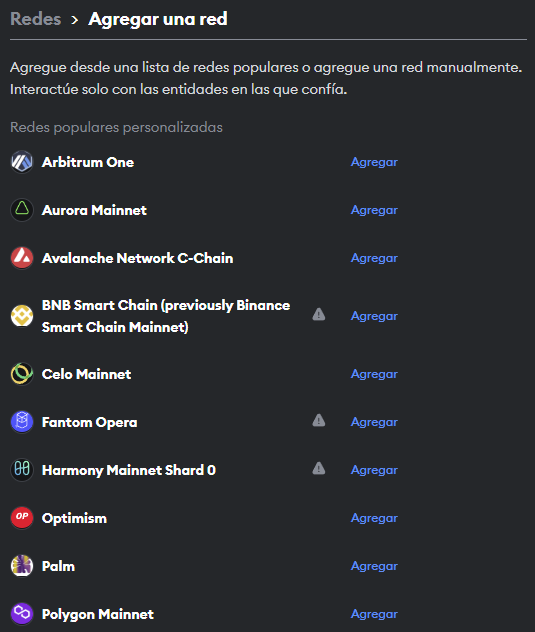
\includegraphics[scale=0.75]{./Ilustraciones/redes.png}\\
    \textbf{Fuente:} Cuenta personal de Metamask al querer agregar una nueva red a día 04/05/2023
\end{figure}
\hfill \break
Las \textbf{transacciones} en una criptomoneda se realizan de forma peer-to-peer (entre 
pares) y se validan a través de un proceso llamado \textbf{minería}. Esta es 
un proceso mediante el cual los usuarios de la red utilizan su poder
de cómputo para resolver problemas matemáticos complejos y validar las 
transacciones en la blockchain. Los usuarios que realizan esta tarea reciben 
recompensas en forma de nuevas unidades de la criptomoneda.\\
\hfill \break
Las criptomonedas se pueden comprar y vender en plataformas de intercambio de 
criptomonedas, y su valor depende de la oferta y la demanda del mercado.\\ 
\hfill \break
Ofrecen varias ventajas, como la descentralización, la transparencia, la 
seguridad y la privacidad, pero también presentan algunos desafíos, como la 
volatilidad del valor y la falta de regulación.\\
\hfill \break
En resumen, las criptomonedas son monedas digitales que utilizan tecnología 
criptográfica y una red descentralizada para asegurar y verificar las 
transacciones. Las criptomonedas se pueden comprar y vender en plataformas de 
intercambio, y su valor depende de la oferta y la demanda del mercado. Las 
criptomonedas como todo en la vida, tiene sus ventajas y sus riesgos.\\
\section{Concepto de NFT}
\label{txt:nft}
Los \textbf{tokens no fungibles} (\textbf{NFT}, por sus siglas en inglés) son 
activos digitales únicos que se utilizan para representar elementos digitales 
como obras de arte, videos, música, juegos, entre otros. A diferencia de las 
criptomonedas tradicionales, los NFT no son intercambiables y cada uno es 
único e irrepetible.\\
\hfill \break
Los NFT se basan en la \textbf{tecnología blockchain} y utilizan contratos 
inteligentes (\textbf{smart contracts}) para garantizar la propiedad y 
autenticidad del activo digital que representan. Los contratos inteligentes 
se utilizan para definir las condiciones y términos de la transacción, y 
garantizan que solo el propietario del NFT tenga derecho a la propiedad del 
elemento digital que representa.\\
\hfill \break
Los NFT se han vuelto muy populares en el mundo del arte digital, ya que 
permiten a los artistas vender sus obras de arte como activos únicos[ 
Por ejemplo, la figura \ref*{fig:opensea-nft}] y garantizar su 
autenticidad y propiedad. También se están utilizando en otros sectores como 
los videojuegos, donde se pueden utilizar para representar objetos y personajes 
únicos [Por ejemplo, la figura \ref*{fig:sorare-nft}].\\
\hfill \break
\begin{figure}[htb!]
    \caption{Muestra de algunos NFT's de la collección de Moonbirds}
    \label{fig:opensea-nft}
    \centering
    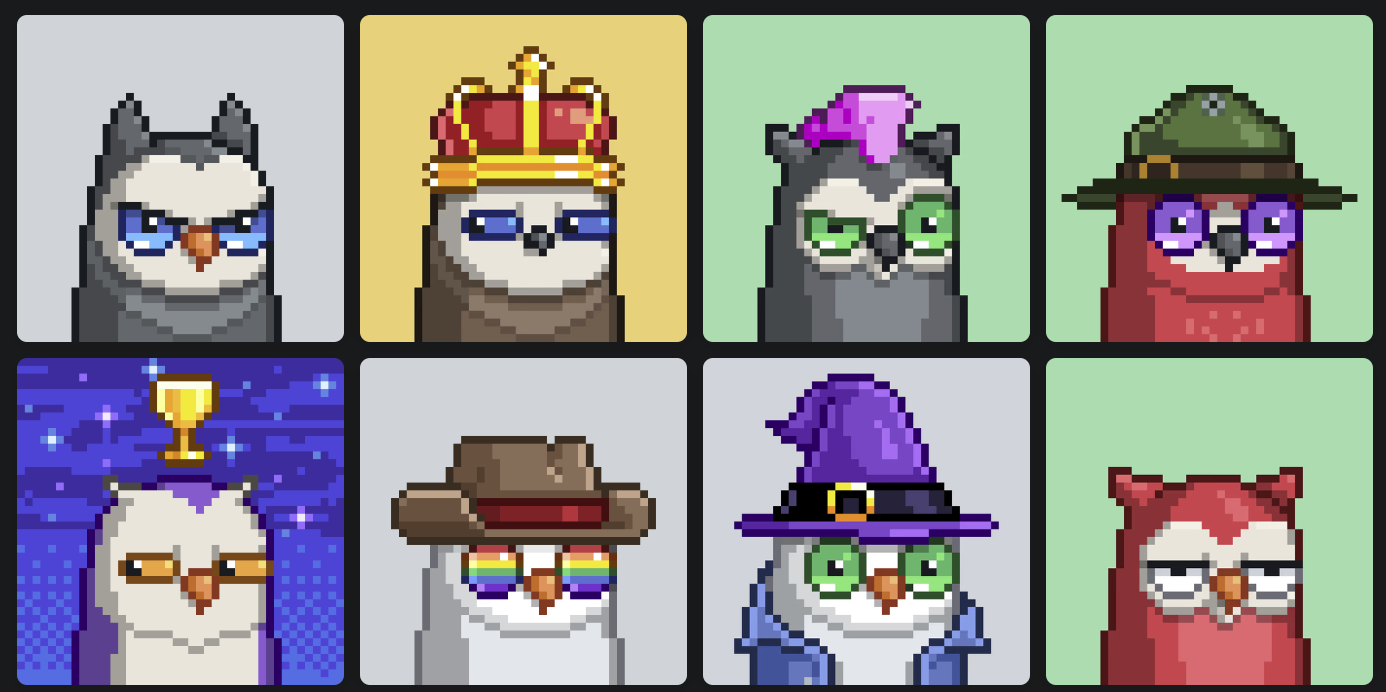
\includegraphics[scale=0.25]{./Ilustraciones/opensea-nft.png}\\
    \textbf{Fuente:} Página de OpenSea [\url{https://opensea.io}]- Collección Moonbirds a día 03/04/2023
\end{figure}
\hfill \break
\begin{figure}[htb!]
    \caption{Muestra de algunos NFT's de la Sorare}
    \label{fig:sorare-nft}
    \centering
    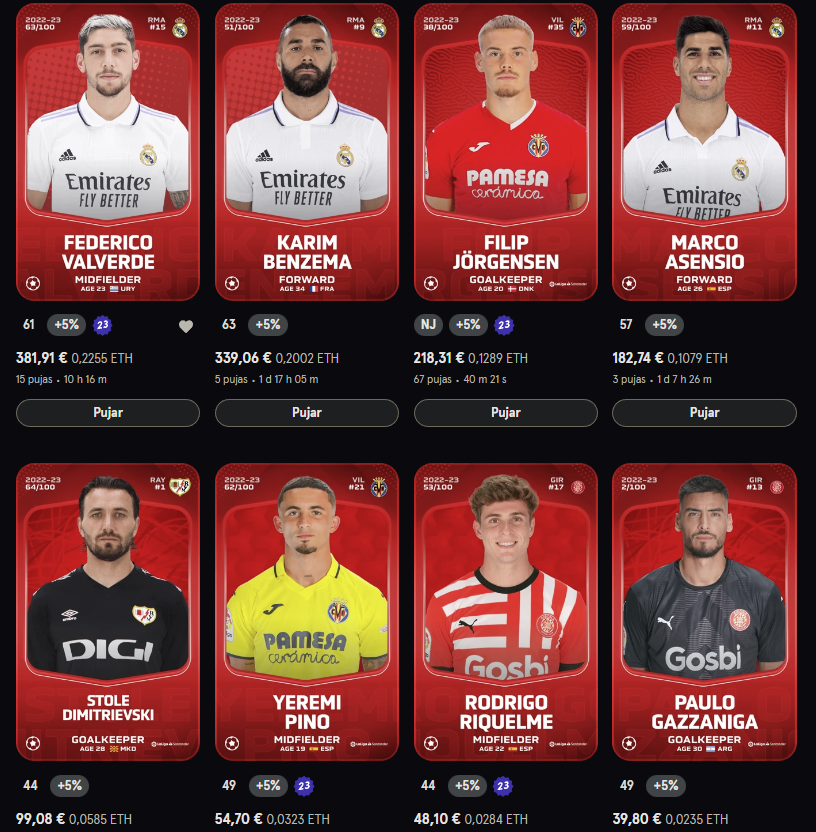
\includegraphics[scale=0.5]{./Ilustraciones/sorare-nft.png}\\
    \textbf{Fuente:} Página de Sorare [\url{https://sorare.com/}]- Sección de mercado con 
    filtros de jugador raro de la Liga Santander a día 03/04/2023
\end{figure}
El valor de un NFT depende de la demanda del mercado y de la percepción del 
valor del activo digital que representa. Los NFT se pueden vender y comprar 
en plataformas especializadas y se utilizan principalmente como activos de 
inversión o de colección.\\
\hfill \break
En resumen, los NFT son activos digitales únicos que se utilizan para 
representar elementos digitales como obras de arte, videos, música, juegos, 
entre otros, y se basan en la tecnología blockchain y contratos inteligentes 
para garantizar la propiedad y autenticidad del activo digital que representan. 
Los NFT se han vuelto muy populares en el mundo del arte digital y se están 
utilizando en otros sectores como los videojuegos\cite{xatakaNFT}.\\
\hfill \break
\newpage
\section{Concepto de CryptoCartera}
\label{txt:wallet}
Una \textbf{criptocartera} es una herramienta que se utiliza para almacenar, 
enviar y recibir criptomonedas. Es similar a una billetera física, pero en 
lugar de contener billetes y monedas, una criptocartera contiene claves 
privadas y públicas que permiten acceder y administrar las criptomonedas.\\
\hfill \break
Cada criptomoneda tiene su propia criptocartera, y hay varios tipos de 
criptocarteras disponibles, incluyendo carteras de hardware, software y en 
línea. Las \textbf{carteras de hardware} (Figura \ref*{fig:ledger}) son dispositivos físicos que se conectan a 
un ordenador y se utilizan para almacenar las claves privadas de manera segura. 
Las \textbf{carteras de software} se descargan en un ordenador o dispositivo 
móvil y se utilizan para almacenar las claves privadas en un archivo cifrado. 
Las \textbf{carteras en línea}(Figura \ref*{fig:coinbase}) se almacenan en la nube y se pueden acceder 
desde cualquier dispositivo con una conexión a internet.
\begin{figure}[htb!]
    \caption{Criptocartera Hardware}
    \centering
    \label{fig:ledger}
    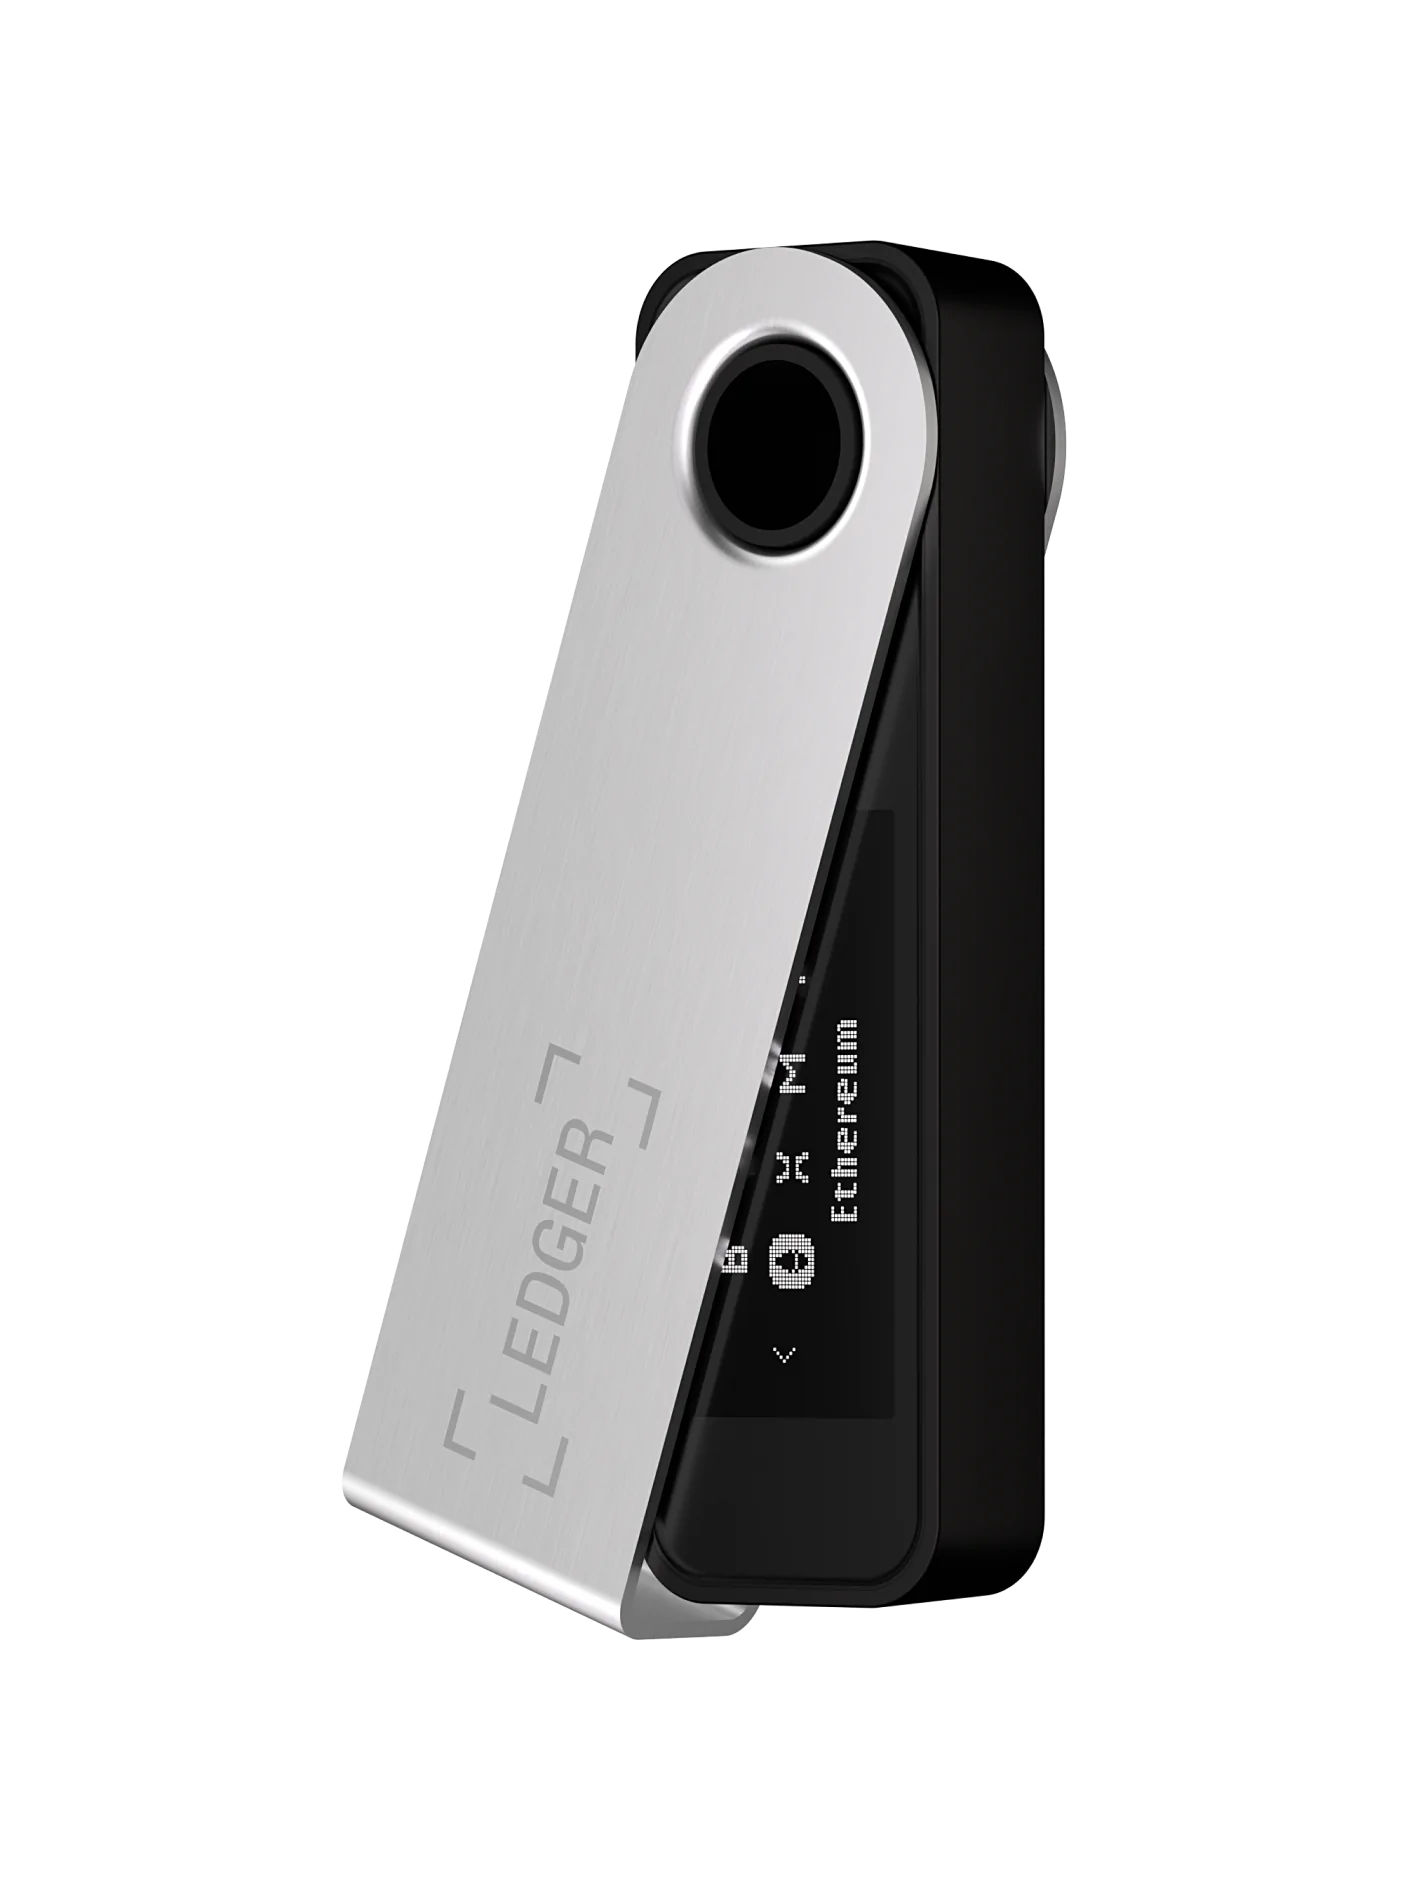
\includegraphics[scale=0.15]{./Ilustraciones/ledger-hardware.png}\\
    \textbf{Fuente:} Página oficial de Ledger [\url{https://shop.ledger.com/products/ledger-nano-s-plus}]
\end{figure}
\hfill \break
\begin{figure}[htb!]
    \caption{Criptocartera Online}
    \label{fig:coinbase}
    \centering
    
\includegraphics[scale=1]{./Ilustraciones/coinbase-logo.png}\\
    \textbf{Fuente:} Logo oficial de Coinbase  [https://www.coinbase.com/es/]
\end{figure}
Las criptocarteras son importantes porque las criptomonedas no se almacenan en 
un lugar centralizado, como un banco, sino que se almacenan en la blockchain de 
la criptomoneda. Por lo tanto, es necesario utilizar una criptocartera para 
acceder y administrar las criptomonedas.\\
\hfill \break
Las criptocarteras también permiten \textbf{enviar y recibir criptomonedas}
de forma segura. Para enviar criptomonedas, se necesita la dirección pública 
de la criptocartera del destinatario. Para recibir criptomonedas, se proporciona 
la dirección pública de la criptocartera al remitente.\\
\hfill \break
En resumen, una criptocartera es una herramienta utilizada para almacenar, 
enviar y recibir criptomonedas. Hay varios tipos de criptocarteras disponibles, 
incluyendo carteras de hardware, software y en línea. Las criptocarteras son 
importantes porque permiten acceder y administrar las criptomonedas, que se 
almacenan en la blockchain de la criptomoneda.
\newpage

\chapter{Estado del Arte}
\section{Industria de la Web 3.0}
La industria de la web3.0 se compone de una variedad de proyectos y empresas
que están trabajando en diferentes aspectos de esta tecnología. Algunos de
estos proyectos incluyen:

\subsection*{Protocolos Blockchain}
Son sistemas que permiten la creación y operación de redes descentralizadas y
seguras. Estos protocolos permiten la creación de aplicaciones
descentralizadas, contratos inteligentes y tokens criptográficos. Los
protocolos blockchain están en constante evolución y crecimiento, y están
impulsados por la comunidad y la colaboración. Algunos de los protocolos
blockchain más populares son Bitcoin, Ethereum, Binance Smart Chain, Polkadot y
Solana.

\subsection*{Criptomonedas}
Son monedas digitales que se basan en la tecnología blockchain y se utilizan
para realizar transacciones en línea de forma segura. Dentro de cada prtocolo
podemos encontrar distintas Criptomonedas, como pueden ser Bitcoin, Etheremun,
Dólares Theter, Solana, Shiba Inu, etc.

\subsection*{Aplicaciones descentralizadas (dApps)}
Este apartado se puede ver de forma más extendida dentro del subcapítulo
\ref{dApps}. \\ Son aplicaciones web que se ejecutan en la blockchain y
utilizan contratos inteligentes para permitir transacciones seguras y sin
intermediarios. Las dApps pueden ser utilizadas para una amplia variedad de
aplicaciones, desde finanzas descentralizadas (DeFi) hasta juegos y redes
sociales. Algunos ejemplos de dApps populares incluyen:
\begin{itemize}
    \item \textbf{Uniswap}: es una plataforma de intercambio descentralizada (DEX)
          que permite a los usuarios intercambiar criptomonedas sin la necesidad de
          intermediarios.
    \item \textbf{Decentraland}: es un mundo virtual descentralizado donde los
          usuarios pueden comprar, vender y construir propiedades virtuales utilizando
          criptomonedas.
    \item \textbf{Brave}: es un navegador web descentralizado que permite a los
          usuarios controlar su privacidad y monetizar su atención en línea.
    \item \textbf{OpenSea}: es un mercado de intercambio descentralizado para
          tokens criptográficos no fungibles (NFT) que permite a los usuarios comprar
          y vender obras de arte digitales, coleccionables y otros activos digitales
          únicos.

\end{itemize}

\subsection*{Conclusión}
La industria de la web3.0 está en constante evolución y crecimiento, y está
impulsada por la comunidad y la colaboración. Los proyectos y empresas en esta
industria están trabajando juntos para construir una internet más segura, justa
y descentralizada.

\section{Páginas principales de la Web 3 en sus distintos ámbitos}
A continuación veremos las \textbf{dApps} más conocidas a día de hoy en los
distintos ámbitos principales[\cite{aplicaciones-descentralizadas}]: Redes
sociales, Servicios de intercambio monetario, servicios de almacenamiento,
Servicios de \textit{streaming} de vídeo y música

\label{dApps}
\subsection*{Redes Sociales Web3}
\label{webs-socialNetworks}
\textbf{Steemit}[\url{https://steemit.com}]: Se ejecuta completamente en la blockchain
Steem. Se describe mejor como una plataforma de recompensa descentralizada que
ayuda a los contribuyentes a monetizar su contenido. Es una alternativa a
Reddit[\url{https://reddit.com}].
\begin{figure}[htb!]
    \caption{Logo de Steemit}
    \label{fig:steemit}
    \centering
    
\includegraphics[scale=0.30]{./Ilustraciones/logos/steemit-logo.png}\\
    \textbf{Fuente:} Steemit[\url{https://steemit.com}]
\end{figure}
Beneficios de las redes sociales descentralizadas. Ninguna autoridad central
que capture datos y los use. Empodera a los usuarios al recompensarlos con
algún tipo de activo. Mejora en las redes sociales de la Web 2.0 en casi todos
los sentidos. Protege la privacidad de los usuarios. Los usuarios deciden qué
quieren compartir y cuándo. Las grandes corporaciones y organizaciones pierden
poder para influir en las grandes corporaciones.

\subsection*{Servicios de intercambio descentralizados}
\label{webs-finanzas}
Cualquiera de estas aplicaciones podrían asociarse a lo que podría ser un
banco, donde podemos introducir dinero en distintas divisas, realizar
transacciones, y el precio de las distintas divisas.

\hfill \break
\textbf{IDEX}: Es un servicio de intercambio descentralizado popular para el
comercio de tokens ERC-20. Proporciona una buena interfaz para los usuarios,
y, cualquier persona con una cartera de ethereum puede comenzar a operar en
la plataforma. Para hacer el mejor uso de IDEX o de cualquier intercambio
descentralizado basado en ethereum, debes utilizar MetaMask.

\hfill \break
\textbf{Coinbase}: Es una plataforma de intercambio de criptomonedas en línea
que permite a los usuarios comprar, vender y almacenar una variedad de
criptomonedas, como Bitcoin, Ethereum, Litecoin, entre otras. Fue fundada en
2012 y se ha convertido en una de las plataformas más populares y utilizadas
en el mundo de las criptomonedas.
\begin{figure}[htb!]
    \caption{Logo de Coinbase}
    \label{fig:coinbase-logo}
    \centering
    
\includegraphics[scale=1]{./Ilustraciones/coinbase-logo.png}\\
    \textbf{Fuente:} Coinbase[\url{https://www.coinbase.com}]
\end{figure}
Además de la plataforma de intercambio, Coinbase también ofrece una billetera
digital integrada para almacenar las criptomonedas y una API para
desarrolladores que deseen integrar las funcionalidades de la plataforma en sus
propias aplicaciones.

\hfill \break
Una de las principales características de Coinbase es su interfaz de usuario
intuitiva y amigable, lo que la hace atractiva tanto para principiantes como
para usuarios avanzados. También se ha destacado por su enfoque en la seguridad
y la protección de los activos de los usuarios, utilizando medidas de seguridad
avanzadas como la autenticación de dos factores y la custodia de criptomonedas.

\hfill \break
Hacer intercambios de criptomonedas de forma descentralizada tiene ciertos
beneficios:
\begin{itemize}
    \item Transacciones más baratas.
    \item Transacciones más rápidas.
    \item Difícil de piratear debido a la naturaleza descentralizada.
    \item Funciona bien con carteras de hardware.
    \item Los usuarios controlan sus propios fondos.
\end{itemize}
Sin embargo, los intercambios descentralizados no están libres de negativos.
Pueden ser difíciles de usar y comprender para los usuarios. Además, la
generación actual de intercambios descentralizados también sufre la falta de
características y funcionalidades. Sin embargo, con el tiempo, veremos la red
descentralizada más avanzada a la par con las contrapartes centralizadas.

\hfill \break
\subsection*{Servicios de Almacenamiento descentralizados}
\label{webs-almacenamiento}
Las siguientes herramientas podrían ser comparadas en la Web2 con Dropbox, Google
Drive o Microsoft OneDrive.

\hfill \break
\textbf{Storj}[\url{https://www.storj.io}]: Storj es una de las principales soluciones de almacenamiento
descentralizado. También es uno de los más antiguos. Con Storj, cualquiera
puede almacenar datos. También es de código abierto y fácil de usar. Cualquiera
puede comenzar a utilizarlo con solo 1-Clic en Inicio. El modelo de pago se
crea alrededor de los usuarios, ya que pueden pagar según lo utilicen. El token
Storj se utiliza para alimentar la plataforma Storj.

\hfill \break
\textbf{Sia}[\url{https://sia.tech}]: Proporciona almacenamiento de forma descentralizada
y también se considera la mayor competencia de Storj. Sia divide el
archivo en treinta segmentos y luego lo distribuye. También encripta el archivo
mientras se transfiere.
\begin{figure}[htb!]
    \caption{Logo de Sia}
    \label{fig:sia}
    \centering
    
\includegraphics[scale=0.25]{./Ilustraciones/logos/sia-logo.jpg}\\
    \textbf{Fuente:} Steemit
\end{figure}
\textbf{IPFS (InterPlanetary File System)}[\url{https://ipfs.tech}]: Es una tecnología de
almacenamiento distribuido que utiliza la red blockchain para almacenar
archivos de manera descentralizada. IPFS permite a los usuarios acceder a los
archivos de forma más rápida y segura, ya que los archivos se almacenan en
múltiples nodos en la red.
\begin{figure}[htb!]
    \caption{Logo de IPFS}
    \label{fig:ipfs}
    \centering
    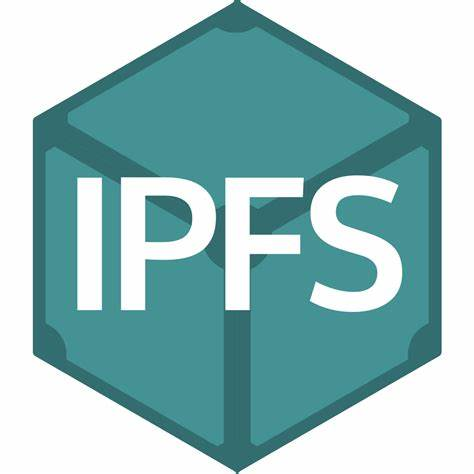
\includegraphics[scale=0.25]{./Ilustraciones/logos/ipfs-logo.jpg}\\
    \textbf{Fuente:} wikipedia [\url{https://es.wikipedia.org/wiki/Sistema_de_archivos_interplanetario}]
\end{figure}
Beneficios de las soluciones de almacenamiento descentralizado Funciona bien en
diferentes plataformas o incluso en soluciones de blockchain. Protege los datos
que se transfieren con cifrado fuerte. Ninguna entidad centralizada, significa
que nadie puede usar los datos. Es barato y funciona bien con tecnologías de
próxima generación como \textbf{IoT (Internet de las cosas)}.

\hfill \break
\subsection*{\textit{Streaming} de Vídeo y Música} \label{webs-streaming} Aquí podríamos comparar con
apliaciones como Twitch[\url{https://www.twitch.tv}],
YouTube[\url{https://www.youtube.com}] o U-beat[\url{https://ubeat.tv}], en el
apartado de \textit{streaming} de vídeo, y aplicaciones web como YouTube
Music[\url{https://music.youtube.com}],
Spotify[\url{https://open.spotify.com/}], o
SoundCloud[\url{https://soundcloud.com}], para el \textit{streaming} de música.

\hfill \break
\textbf{LivePeer}[\url{https://livepeer.org/es}]: Proporciona un servicio de
transmisión, es de código abierto y apunta a construir una stack de streaming
para la Web 3.0.

\hfill \break
\textbf{LBRY}[\url{https://lbry.com}]: Biblioteca digital
descentralizada que alberga diferentes formas de contenido. Como usuario,
puedes leer, ver y jugar en la plataforma. Esto significa que admite libros,
música y videos. Es uno de los proyectos Web 3.0 más antiguos.

\hfill \break
\textbf{UjoMusic}[\url{https://www.mesh.xyz}]: Plataforma de música donde los
creadores pueden cargar su música y distribuirla sin problemas de derechos de
autor o royalty. Las criptomoneda y los contratos inteligentes lo potencian.

\hfill \break
\textbf{Audius}[\url{https://audius.co}]: Es una plataforma de música
descentralizada que permite a los artistas compartir su música y monetizarla.
Los usuarios pueden escuchar música de forma gratuita. Esta aplicación es la
que pretende reemplazar a Spotify dentro del mundo descentralizado.

\begin{figure}[htb!]
    \caption{Logo de Audius}
    \label{fig:audius}
    \centering
    
\includegraphics[scale=0.25]{./Ilustraciones/logos/Audius.jpg}\\
    \textbf{Fuente:} Ecosystem.ipfs [\url{https://ecosystem.ipfs.tech/project/audius/}]
\end{figure}

\hfill \break
Los creadores de contenido pueden trabajar en un entorno transparente. odos
tienen las mismas oportunidades de promover su trabajo. Los problemas de
derechos de autor serán insignificantes gracias a los contratos inteligentes y
no hay autoridad central, por lo tanto no será una política absurda para los
streamers y los creadores de contenido.

\subsection*{Navegadores descentralizados}
\label{webs-browsers}
Teniendo en cuenta los navegadores más utilizados en estos últimos 5 años [Figura \ref{fig:browser}],
podemos ver que las comparaciones son abrumadoras, teniendo Google Chrome casi un 63\% del mercado,
siguiéndole Safari, Mozilla Firefox y Samsung Internet.
Por lo que cualquiera de los siguientes navegadores no pueden competir con este,
aunque tienen sus beneficios al estar implementando la tecnología blockchain.

\hfill \break
\textbf{Brave Browser}[\url{https://brave.com/es/}]:
Brave tiene que ver con la privacidad donde los usuarios no son el producto.
El navegador viene preinstalado con el bloqueador de anuncios. También permitirá
a los usuarios vender sus datos a cambio de la criptomoneda, BAT, la cual pueder
ser usada para diversos propósitos, como pueden ser hacer Staking, ser cambiadas por
otra Criptomoneda, o venderla para conseguir divisa.

\begin{figure}[htb!]
    \caption{logos de Brave}
    \label{fig:brave}
    \centering
    
\includegraphics[scale=0.1]{./Ilustraciones/logos/brave-logo.png}\\
    \textbf{Fuente:} logos.Wine
\end{figure}

\textbf{Breaker Browser}[\url{https://github.com/beakerbrowser}]:
Es un navegador web de próxima generación basado en
punto a punto (P2P)\footnote{ red de computadoras en la que todos los aspectos
    (o la mayoría de ellos) funcionan con una serie de nodos que se comportan de
    la misma manera entre sí y sin clientes ni servidores fijos\cite{p2p}}.
Es un lugar donde cualquiera puede unirse, compartir y
sobrecargar sus aplicaciones. Es una herramienta creativa que puede ser
explorada por cualquier persona. Es un navegador web 3.0.

\hfill \break
Beneficios de los navegadores descentralizados: Los usuarios pueden navegar de
forma privada por internet.\\ Ninguna o menor cantidad de lagunas de seguridad.
\\ Los usuarios pueden vender sus datos a una organización y recibir pagos.
Rápido y seguro.
\begin{figure}[htb!]
    \caption{Navegadores más usados entre 2018 y 2023}
    \label{fig:browser}
    \centering
    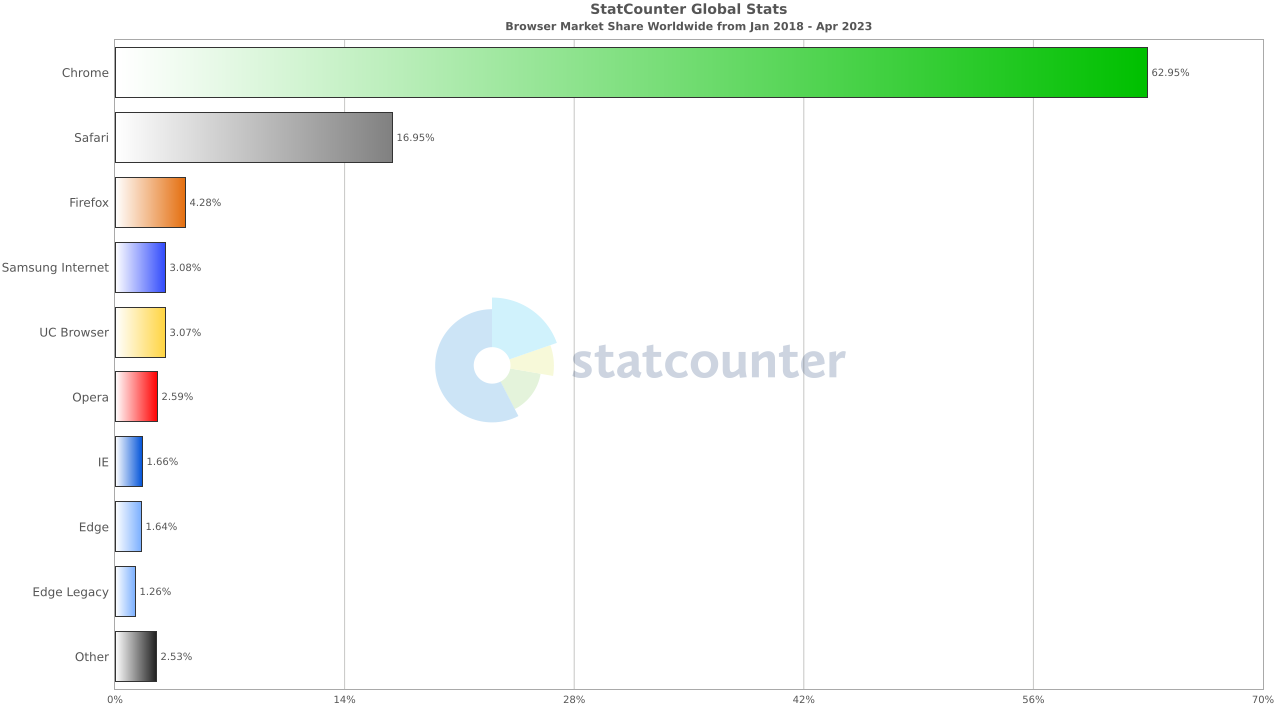
\includegraphics[scale=0.5]{./Ilustraciones/StatCounter-browser-ww-monthly-201801-202304-bar.png}\\
    \textbf{Fuente:} StatCounter [\url{https://gs.statcounter.com/browser-market-share#monthly-201801-202304-bar}]
\end{figure}

\section{Conclusión}
La web3 se está desarrollando rápidamente y se espera que cambie la forma en
que interactuamos en línea. Con la tecnología blockchain y los contratos
inteligentes, la web3 permitirá aplicaciones descentralizadas, transacciones
financieras sin intermediarios y la propiedad verdadera de los datos. Algunos
de los protocolos blockchain más populares para la web3 incluyen Ethereum,
Polkadot y Solana.

\hfill \break
Las criptomonedas continúan siendo una fuerza importante en el mercado
financiero global. Bitcoin sigue siendo la criptomoneda más grande y popular,
pero hay muchas otras criptomonedas importantes, como Ethereum, Binance Coin y
Cardano. La capitalización total del mercado de criptomonedas ha aumentado
significativamente en los últimos años, llegando a más de 2 billones de
euros[Figura \ref{fig:capit}] en abril de 2021.
\begin{figure}[htb!]
    \centering
    \caption{Capitalización total del mercado de criptomonedas entre abri del 2017 y mayo de 2023}
    \label{fig:capit}
    \centering
    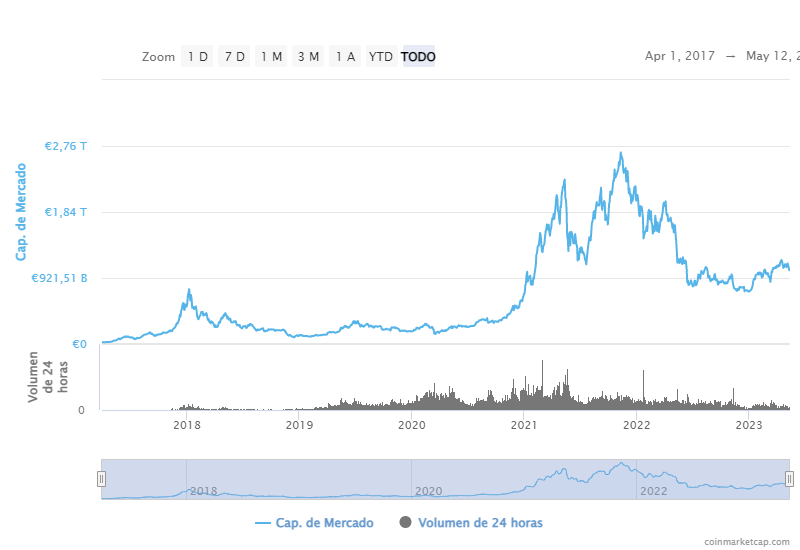
\includegraphics[scale=0.45]{./Ilustraciones/CoinMarketCap chart.png}\\
    \textbf{Fuente:} CoinMarketCap [\url{https://coinmarketcap.com/es/charts/}]
\end{figure}
\hfill \break
Los NFTs se han convertido en un nuevo mercado emocionante en la web3. Las ventas de
NFTs han aumentado significativamente en desde 2020, con algunos NFTs vendiéndose por
decenas de miles de dólares.

\hfill \break
La regulación de las criptomonedas y los NFTs sigue siendo un tema importante.
A medida que estos mercados crecen, los reguladores de todo el mundo están
considerando cómo regularlos para proteger a los inversores y prevenir el
fraude. En algunos países, como China, se han tomado medidas más drásticas para
prohibir las criptomonedas y las transacciones de NFTs.
\newpage
\chapter{Recursos y tecnologías}
\label{recursos}
En este capítulo se tratan los recursos y las tecnologías empleadas para el
diseño y desarrollo de la aplicación Web.

\section{Angular}
\label{Angular}
Angular[\url{https://angular.io}] es un framework de desarrollo web para crear
aplicaciones de una sola página (SPA) y aplicaciones web dinámicas. Fue
desarrollado por Google y se basa en el lenguaje de programación TypeScript.
\begin{figure}[htb!]
    \centering
    \caption{Logo de Angular}
    \label{fig:angular-logo}
    \centering
    
\includegraphics[scale=0.35]{./Ilustraciones/logos/Angular Logo.png}\\
    \textbf{Fuente:} Página oficial de Angular [\url{https://angular.io}]
\end{figure}
\hfill \break
Angular proporciona una estructura sólida y coherente para el desarrollo de
aplicaciones web complejas, lo que permite a los desarrolladores construir
aplicaciones de alta calidad y escalables de manera más rápida y eficiente.
Algunas de las características clave de Angular incluyen:

\textbf{Inyección de dependencias}: Permite que los componentes se comuniquen entre sí
de manera eficiente.

\textbf{Binding de datos bidireccional}: Facilita la actualización automática de la
interfaz de usuario en tiempo real.

\textbf{Directivas}: Permite crear componentes personalizados y hacer uso de componentes
predefinidos.

\textbf{Servicios}: Permite compartir datos y lógica de aplicación entre los
componentes.

Angular también viene con una amplia variedad de herramientas y bibliotecas
adicionales, como Angular CLI y Angular Material, que ayudan a los
desarrolladores a crear aplicaciones web robustas y de alta calidad.
\begin{figure}[htb!]
    \centering
    \caption{Logo de Angular Material}
    \label{fig:angularMat-logo}
    \centering
    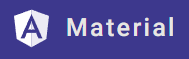
\includegraphics[scale=1]{./Ilustraciones/logos/Angular-Mat Logo.png}\\
    \textbf{Fuente:} Página oficial de Angular Material [\url{https://material.angular.io}]
\end{figure}
\hfill \break
Se ha hecho uso de un algunos componentes de Angular Material, como son:

Material Table
    [\url{https://v5.material.angular.io/components/table/overview}], junto con
Paginator:\\ El \textbf{componente mat-table} proporciona una tabla de datos de
estilo Material Design que se puede utilizar para mostrar filas de datos. \\ El
\textbf{componente mat-paginator} Proporciona navegación para la información
paginada, normalmente utilizada con una tabla.
\begin{figure}[htb!]
    \centering
    \caption{Muestra de tabla y paginator en Trabajo propio}
    \label{fig:tabla}
    \centering
    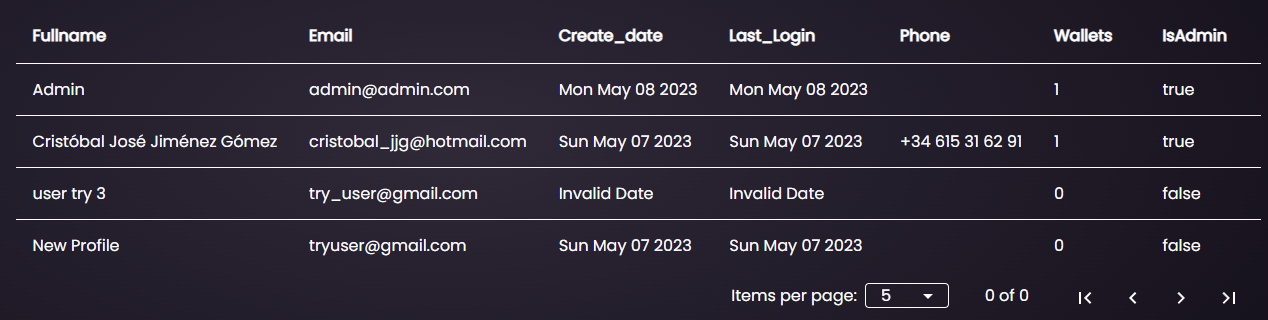
\includegraphics[scale=0.5]{./Ilustraciones/table-paginator.png}\\
    \textbf{Fuente:} Trabajo Propio en la zona de admin [\url{https://tft-galeria-nft-web3.vercel.app/admin/users}]
\end{figure}
\hfill \break

\section{Express.JS}
\label{ExpressJS}
Como dicen en su propia página web, "ExpressJS es una opción rápida, sin
opiniones y minimalista para Node.js."\\ Es un popular marco de aplicación web
para Node.js que simplifica el proceso de creación de aplicaciones web y APIs
(interfaces de programación de aplicaciones). Es una capa delgada sobre Node.js
que proporciona una variedad de características y herramientas para crear
aplicaciones web y APIs de manera rápida y eficiente.
\begin{figure}[htb!]
    \centering
    \caption{Logo de ExpressJS}
    \label{fig:express-logo}
    \centering
    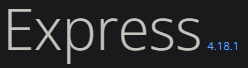
\includegraphics[scale=0.5]{./Ilustraciones/logos/ExpressJS.png}\\
    \textbf{Fuente:} Página oficial de ExpressJS [\url{http://expressjs.com}]
\end{figure}
\hfill \break

ExpressJS es un marco minimalista que proporciona una estructura básica para
construir aplicaciones web, pero permite a los desarrolladores agregar
funcionalidad adicional utilizando middleware y complementos. ExpressJS también
proporciona un enrutamiento simple y flexible, lo que facilita la creación de
rutas para diferentes páginas y recursos.

Además, ExpressJS es altamente personalizable y se integra fácilmente con otros
módulos y herramientas de Node.js, lo que lo convierte en una opción popular
para construir aplicaciones web y APIs.

\section{API's}
\label{APIs}
\subsection{Firebase}
\label{Firebase-desglosado}
Firebase es una plataforma de desarrollo de aplicaciones móviles y web que
ofrece una variedad de herramientas y servicios en la nube para ayudar a los
desarrolladores a crear, mejorar y escalar aplicaciones.
\begin{figure}[htb!]
    \centering
    \caption{Logo de Firebase}
    \label{fig:firebase-logo}
    \centering
    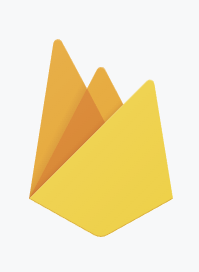
\includegraphics[scale=0.35]{./Ilustraciones/logos/Firebase.png}\\
    \textbf{Fuente:} Página oficial de Firebase [\url{https://firebase.google.com/?hl=es}]
\end{figure}
\hfill \break
Firebase fue adquirido por Google en 2014 y desde entonces ha evolucionado para
ofrecer una amplia gama de servicios, incluyendo:
\begin{itemize}
    \item Autenticación de usuarios[Capítulo \ref{autenticacion}]: permite a los
          desarrolladores agregar fácilmente funciones de registro, inicio de sesión y
          autenticación a sus aplicaciones.
    \item Almacenamiento en la nube[Capítulo \ref{almacenamiento}]: proporciona
          almacenamiento en la nube para archivos y datos de aplicaciones.
    \item Base de datos en tiempo real: una base de datos en tiempo real en la nube que
          permite a los desarrolladores crear aplicaciones en tiempo real con
          actualizaciones automáticas y en tiempo real.
    \item Alojamiento de aplicaciones web: permite a los desarrolladores alojar sus
          aplicaciones web en los servidores de Firebase.
    \item Notificaciones push: permite enviar notificaciones push a los usuarios de la
          aplicación.
    \item Analítica de aplicaciones: proporciona análisis de usuarios y datos de uso de
          la aplicación.
\end{itemize}

Para este proyecto no se ha hecho uso de todas las utilidades, solamente de:

\subsubsection{Autenticación de usuarios}
\label{autenticacion} Se ha hecho uso de esta
utilidad debido a que nos proporciona una forma sencilla de registrar usuarios,
hacer que estos inicien sesión, y que puedan cerrar sesión de una forma simple.
Además, y como veremos en las conclusiones y trabajo futuro [Capítulo \ref{trabajo-futuro}],
nos permite hacer uso de la autenticación de Google, lo que nos permite tener
una mayor seguridad en el inicio de sesión de los usuarios.
\begin{figure}[htb!]
    \centering
    \caption{Tabla de autenticación proporcionada por Firebase}
    \label{fig:firebase-autenticacion}
    \centering
    \includegraphics[scale=0.65]{./Ilustraciones/autenticación.png}\\
    \textbf{Fuente:} Consola de Firebase, apartado de Autenticación
\end{figure}
\hfill \break

\subsubsection{Almacenamiento en la nube}
\label{almacenamiento}
Se ha hecho uso de esta utilidad debido a que nos proporciona una base de datos
en la nube, lo que nos permite tener una mayor seguridad en el almacenamiento de
los datos de los usuarios, y de la aplicación en general.
En este caso, guardamos 3 tipos de datos:
\begin{itemize}
    \item Los \textbf{usuarios} registrados, con la información del correo, si es
          administrador, el nombre, el apellido, su número de móvil, su nombre de
          usuario, que está compuesto por el inicio del correo y su primer nombre, y las
          carteras que este ha agregado.
    \item Las \textbf{colecciones} que se mostrarán de NFT's, que contienen las
          direcciones de las colecciones para poder acceder a las mismas, la url de la
          colleción, el nombre real y la foto de la marca.
    \item También se ha hecho un apartado para \textbf{mensajes}, el cual contiene
          mensajes qeu hand ejado los usuarios con intenciones de mejora. Este documento
          contiene el correo del usuario que lo ha mandado, el mensaje, y un asunto.
\end{itemize}

\begin{figure}[htb!]
    \centering
    \caption{Conjunto de colecciones y documentos proporcionada por Firebase}
    \label{fig:firebase-almacenamiento}
    \centering
    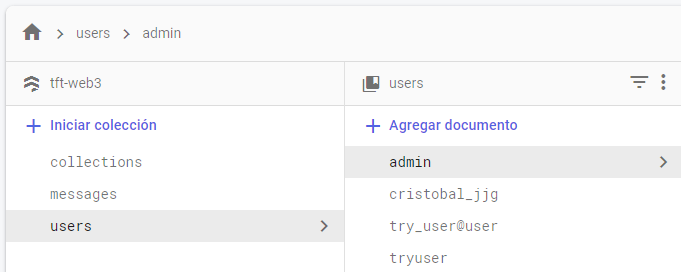
\includegraphics[scale=0.75]{./Ilustraciones/almacenamiento.png}\\
    \textbf{Fuente:} Consola de Firebase, apartado de Firestore Database
\end{figure}

\subsection{Alchemy}
\label{Alchemy-desglosado}
Alchemy es una plataforma de desarrollo con soporte multicadena y con alcance
global, pensada en facilitar el desarrollo de aplicaciones descentralizadas
(DApps). Su principal objetivo es ofrecer todo lo que los desarrolladores
necesitan para construir y hacer realidad la Web3.[\cite{alchemy}]
\begin{figure}[htb!]
    \centering
    \caption{Logo de Alchemy}
    \label{fig:alchemy-logo}
    \centering
    
\includegraphics[scale=0.5]{./Ilustraciones/logos/alchemy-logo.png}\\
    \textbf{Fuente:} Página oficial de Alchemy [\url{https://www.alchemy.com}]
\end{figure}
\hfill \break

Su relevancia en el sector le ha válido ser reconocida como el “AWS de la
Web3”, manejando más de 10 millones de usuarios, movilizando más de 100 mil
millones de dólares en activos digitales y con un concurrencia de más de 100
mil millones de requests, lo que le ha llevado a tener una valoración de
mercado de más 10 mil millones de dólares.\\

La intención de la plataforma es permitir que las aplicaciones puedan
evolucionar rápidamente para dar respuesta a las necesidades de los usuarios,
sin que esto implique la puesta en marcha de tales mejoras. Así, los
desarrolladores se pueden enfocar en lo realmente importante: diseñar y
codificar estas nuevas soluciones, confiando en que la plataforma tendrá la
flexibilidad necesaria para respaldar estos nuevos diseños y permitir que los
usuarios puedan explorarlos.

\subsection{Moralis}
\label{Moralis-desglosado}
Moralis [\url{https://moralis.io}] es una plataforma de infraestructura
blockchain de la web3 que proporciona herramientas y servicios para
desarrolladores que construyen aplicaciones descentralizadas (dApps) en la
cadena de bloques Ethereum. Ofrece una amplia gama de herramientas, incluyendo
APIs y nodos de red, para que los desarrolladores puedan interactuar con
Ethereum de manera eficiente y escalable.
\begin{figure}[htb!]
    \centering
    \caption{Logo de Moralis}
    \label{fig:moralis-logo}
    \centering
    
\includegraphics[scale=0.5]{./Ilustraciones/logos/Moralis-logo.png}\\
    \textbf{Fuente:} Página oficial de Moralis [\url{https://moralis.io}]
\end{figure}
\hfill \break

Moralis también proporciona herramientas de desarrollo para que los
desarrolladores puedan construir dApps en la cadena de bloques Ethereum de
manera más fácil y rápida. La plataforma es utilizada por una gran cantidad de
proyectos y empresas en el espacio de la web3, y es conocida por su facilidad
de uso y eficiencia en la construcción de aplicaciones descentralizadas en la
cadena de bloques Ethereum.

Entre estas empresas, podemos encontrar algunas antes nombradas, como son
Metamask[\url{https://metamask.io}] o Polygon
    [\url{https://polygon.technology}]

\section{IDE - Visual Studio Code}
\label{VSCode}
Visual Studio Code (también conocido como VS Code)
[\url{https://code.visualstudio.com}] es un editor de código fuente
desarrollado por Microsoft, que es compatible con múltiples lenguajes de
programación. Está disponible de manera gratuita para Windows, Linux y macOS, y
es muy popular entre los desarrolladores por su facilidad de uso, flexibilidad
y personalización.
\begin{figure}[htb!]
      \centering
      \caption{Logo de Visual Studio Code}
      \label{fig:vscode-logo}
      \centering
      
\includegraphics[scale=0.1]{./Ilustraciones/logos/vscode-logo.png}\\
      \textbf{Fuente:} Iconduck [\url{https://iconduck.com/icons/102490/file-type-vscode}]
\end{figure}
\hfill \break

VS Code incluye características útiles como resaltado de sintaxis,
autocompletado de código, depuración de código en vivo, integración con control
de versiones y herramientas de construcción y despliegue de aplicaciones.
Además, los usuarios pueden personalizar el editor con extensiones y temas para
satisfacer sus necesidades específicas de programación.

VS Code es muy popular en el desarrollo web y en la construcción de
aplicaciones para la web3 y las criptomonedas.

Se han utilizado algunas extensiones básicas para el desarrollo web como son:
\begin{itemize}
      \item Angular Language Service [\url{https://angular.io/guide/language-service}]
      \item Auto Close Tag
                  [\url{https://marketplace.visualstudio.com/items?itemName=formulahendry.auto-close-tag}]
      \item Auto Rename Tag
                  [\url{https://marketplace.visualstudio.com/items?itemName=formulahendry.auto-rename-tag}]
      \item Console Ninja
                  [\url{https://marketplace.visualstudio.com/items?itemName=WallabyJs.console-ninja}]
      \item IntelliCode
            [\url{https://marketplace.visualstudio.com/items?itemName=VisualStudioExptTeam.vscodeintellicode}]
      \item GitHub Copilot Nightly
                  [\url{https://marketplace.visualstudio.com/items?itemName=GitHub.copilot-nightly}]
      \item Prettier - Code formatter
                  [\url{https://marketplace.visualstudio.com/items?itemName=esbenp.prettier-vscode}]
      \item SCSS Formatter
                  [\url{https://marketplace.visualstudio.com/items?itemName=sibiraj-s.vscode-scss-formatter}]
      \item VSCode-pdf
            [\url{https://marketplace.visualstudio.com/items?itemName=tomoki1207.pdf}]
\end{itemize}

\section{Trello}
\label{Trello}
Trello es una herramienta de gestión de proyectos basada en la nube, que
permite a los usuarios organizar tareas y proyectos en tableros visuales y
colaborativos. Fue lanzado en 2011 y se ha vuelto muy popular entre equipos de
trabajo de diversas industrias y tamaños.
\begin{figure}[htb!]
    \centering
    \caption{Logo de Trello}
    \label{fig:trello-logo}
    \centering
    
\includegraphics[scale=0.05]{./Ilustraciones/logos/trello.1024x1024.png}\\
    \textbf{Fuente:} Iconduck [\url{https://iconduck.com/icons/95002/trello}]
\end{figure}
\hfill \break
Trello utiliza un sistema de tableros que representan los diferentes proyectos
o áreas de trabajo, y dentro de cada tablero, los usuarios pueden crear listas
de tareas y tarjetas que representan cada tarea o actividad. Estas tarjetas
pueden contener información como descripciones, listas de verificación,
etiquetas, fechas de vencimiento, comentarios y archivos adjuntos.

Además, Trello permite la colaboración entre equipos de trabajo, ya que los
miembros pueden comentar en las tarjetas, asignar tareas a otros miembros,
establecer fechas de vencimiento y recibir notificaciones de actualizaciones.
Trello también se integra con otras herramientas populares de productividad,
como Slack, Google Drive y Jira, lo que lo hace aún más útil para equipos de
trabajo que utilizan diferentes herramientas.

\section{Figma}
\label{Figma}
Figma es una herramienta de diseño gráfico en línea que se utiliza para crear
interfaces de usuario, diseños de sitios web, aplicaciones móviles y otros
proyectos digitales. Fue lanzado en 2016 y se ha vuelto muy popular en la
industria del diseño debido a su capacidad para trabajar en tiempo real y
permitir la colaboración en tiempo real entre los miembros del equipo.
\begin{figure}[htb!]
    \centering
    \caption{Logo de Figma}
    \label{fig:figma-logo}
    \centering
    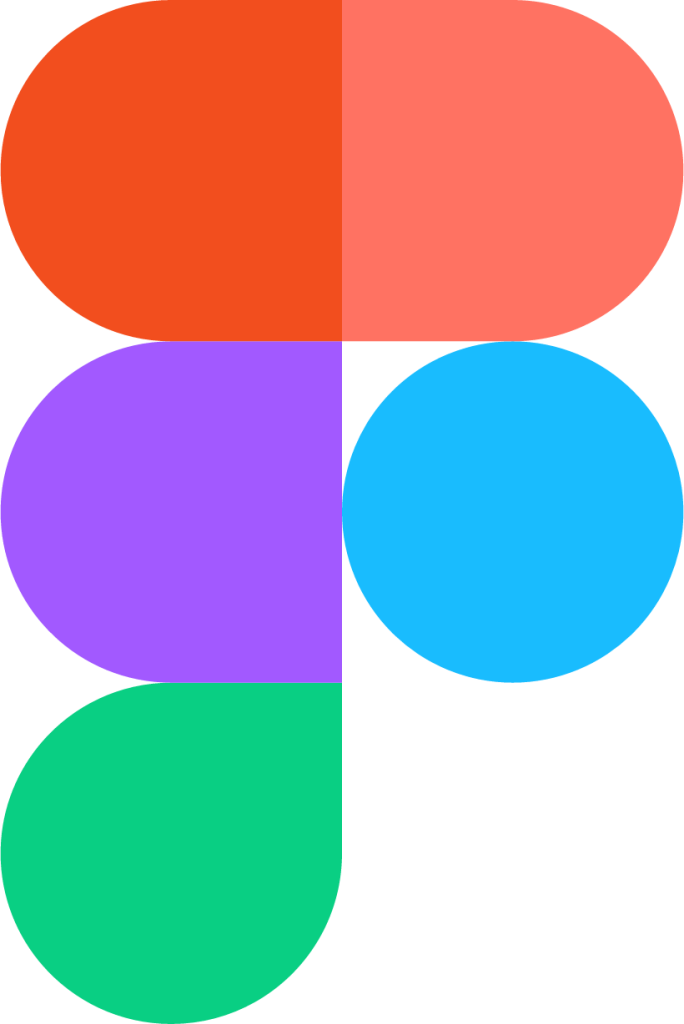
\includegraphics[scale=0.05]{./Ilustraciones/logos/figma.684x1024.png}\\
    \textbf{Fuente:} Iconduck [\url{https://iconduck.com/icons/39864/figma}]
\end{figure}
Figma nos permite crear diseños con herramientas como vectores,
formas, capas, texto y efectos, entre otras. También tiene características como
prototipado y animación, lo que lo hace ideal para diseñar interfaces interactivas.

Además, Figma es una herramienta basada en la nube, lo que significa que todos
los archivos se guardan en línea y se pueden acceder desde cualquier lugar con
conexión a Internet. Esto permite la colaboración en tiempo real entre los
miembros del equipo, ya que varios diseñadores pueden trabajar en un proyecto
simultáneamente y realizar cambios que se actualizan en tiempo real.
\newpage
\chapter{Metodología}
\section{Marco de Trabajo SCRUM}\label{Scrum}

Para la creación de la aplicación Web3 se ha seguido un marco de trabajo
inspirado en \textbf{SCRUM} para un desarrollo ágil. Este marco de trabajo está
fundamentado por la existencia de etapas de tiempo previamente establecidas
donde se enfoca la carga de trabajo, consiguiendo un producto mínimamente
viable en cada una de ellas. Estas etapas de tiempo se conocen por el nombre de
Sprints, y cada uno de ellos se divide en diferentes fases: planificación del
Sprint, realización del Sprint, con reuniones diarias, y retrospectiva del
Sprint. En la Figura \ref*{fig:scrum-imagen} se muestra el flujo de trabajo que
se suele seguir en la metodología SCRUM.

\begin{figure}[htb!]
    \centering
    \caption{Metodología SCRUM} \label{fig:scrum-imagen}
    \centering
    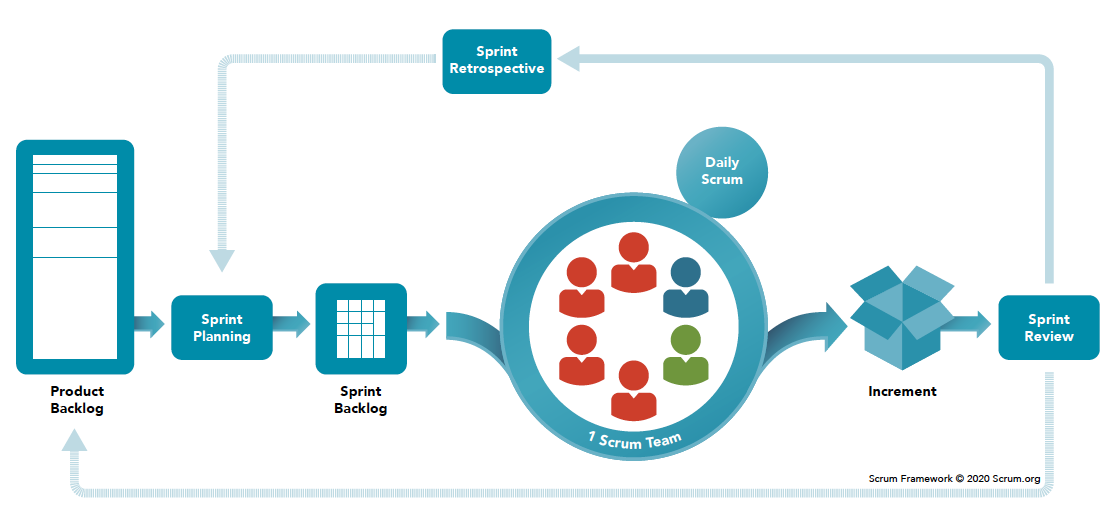
\includegraphics[scale=0.4]{./Ilustraciones/scrum.png}\\
    \textbf{Fuente:} www.scrum.org [\url{https://www.scrum.org/learning-series/what-is-scrum}]
\end{figure}

\textbf{Planificación del Sprint}: En esta fase, se definen
los objetivos del sprint, identifican las tareas necesarias para cumplir esos
objetivos y determinan la cantidad de trabajo que se puede realizar en el
sprint.

\textbf{Sprint}: Esta es la fase en la que se realiza el trabajo. Durante el sprint, se
trabaja en las tareas definidas en la planificación del sprint
para lograr los objetivos establecidos.

\textbf{Reunión diaria}: En esta fase, el equipo Scrum se reúne diariamente para revisar
el progreso del trabajo, identificar cualquier problema y hacer ajustes
necesarios para alcanzar los objetivos del sprint.

\textbf{Revisión del Sprint}: Al final del sprint, el equipo Scrum se reúne para revisar
el trabajo completado y demostrar los resultados a los interesados. Esto ayuda
a identificar los logros y también a las áreas donde se pueden mejorar.

\textbf{Retrospectiva del Sprint}: En esta fase, el equipo Scrum reflexiona sobre el
sprint anterior y discute qué se hizo bien y qué se puede mejorar en el próximo
sprint.

\textbf{Planificación de lanzamiento}: Si se han completado múltiples sprints, el equipo
Scrum se reúne para planificar la entrega del producto final al cliente.

A la hora de hacerlo, al no tener un "equipo", sino ser únicamente una persona,
la \textbf{planificación} del sprint se realizaba mediante el uso de
Trello[\ref{Trello}], añadiendo tareas, y colocando sus respectivos "tests",
que en su mayoría son validaciones por parte de personas externas.

La \textbf{realización del sprint} se realizaba en diferentes apartados, los
cuales son: \\

La parte de \textbf{diseño} realizado en Figma[Sección \ref{Figma}]
\begin{itemize}
    \item Diseño de componentes
    \item Diseño de páginas con los componentes diseñados
\end{itemize}

La parte de \textbf{desarrollo} realizado en Figma[Sección \ref{VSCode}]
haciendo uso de las distintas herramientas antes mencionadas[Capítulo
        \ref{recursos}].
\begin{itemize}
    \item Desarrollo de la página para poder colocar los componentes
    \item Desarrollo de los componentes e insertarlos de forma adecuada en la página
\end{itemize}

La parte de \textbf{validación} realizado con Lighthouse[Sección
        \ref{lighthouse}] y SonarQube[Sección \ref{sonarqube}]
\begin{itemize}
    \item Siguiendo el consejo antes mencionado de SonarQube, se pasaba el test antes de
          hacer un \textit{push}, comprobando la posible existencia de Code Smells, bugs,
          vulnerabilidades, etc.
    \item A la hora de pasar la validación de Lighthouse se hizo cada vez que se hacía un
          \textit{merge} a la rama principal, se pasaba este test para ver las posibles
          fallas de accesibilidad que tenía la página en ese momento y poder
          solucionarlas.\end{itemize}
\newpage
\chapter{Análisis y Diseño}
\newpage
\chapter{Desarrollo}
\newpage
%----Fin del Desarrollo----%

%----Evaluación y resultados----%
\chapter{Evaluación y resultados}

%----Conclusiones y trabajo futuro----%

\chapter{Conclusiones y trabajo futuro}
%\input{Conclusiones.tex}
CAPÍTULO OBLIGATORIO

Resultados, grado de consecución de los objetivos, posibles extensiones
\newpage

\bibliography{bib.bib}

\end{document}